\documentclass[11pt,a4paper]{report}
\usepackage[portuguese]{babel}
\usepackage[utf8]{inputenc} % define o encoding usado texto fonte (input)--usual "utf8" ou "latin1
\usepackage{graphicx} %permite incluir graficos, tabelas, figuras
\usepackage{subcaption}
\usepackage[title]{appendix}
\usepackage{listings}
\usepackage{color}
\usepackage{multicol}
\usepackage{indentfirst}
\usepackage{hyperref}
\usepackage{amsmath}
\usepackage{amssymb}
\usepackage{float}
\usepackage{enumerate}
\usepackage[shortlabels]{enumitem}
\usepackage[T1]{fontenc}
\usepackage{hyperref}
\usepackage[margin=1in]{geometry}
\usepackage{array}
\usepackage[table]{xcolor}
\usepackage{tcolorbox}
\usepackage{longtable}
\usepackage{tcolorbox}

\definecolor{headerblue}{RGB}{0, 102, 204}
\definecolor{headerblack}{RGB}{0, 0, 0}
\definecolor{lightgray}{rgb}{0.95,0.95,0.95}
\definecolor{mygreen}{rgb}{0,0.6,0}
\definecolor{mygray}{rgb}{0.5,0.5,0.5}
\definecolor{mymauve}{rgb}{0.58,0,0.82}

\hypersetup{
    colorlinks=true,
    linkcolor=blue,
    urlcolor=black,
    }
    
\usepackage{bera}% optional: just to have a nice mono-spaced font

\definecolor{eclipseStrings}{RGB}{42,0.0,255}
\definecolor{eclipseKeywords}{RGB}{127,0,85}

\lstset{ %
  backgroundcolor=\color{white},   % choose the background color
  basicstyle=\footnotesize,        % size of fonts used for the code
  breaklines=true,                 % automatic line breaking only at whitespace
  captionpos=b,                    % sets the caption-position to bottom
  commentstyle=\color{mygreen},    % comment style
  escapeinside={\%*}{*)},          % if you want to add LaTeX within your code
  keywordstyle=\color{blue},       % keyword style
  stringstyle=\color{mymauve},     % string literal style
}

\lstdefinestyle{phpstyle}{
    language=PHP,
    basicstyle=\ttfamily\small,
    keywordstyle=\bfseries,
    commentstyle=\itshape,
    stringstyle=\ttfamily,
    numbers=left,
    numberstyle=\tiny,
    stepnumber=1,
    numbersep=8pt,
    frame=single,
    rulecolor=\color{black!30},
    breaklines=true,
    breakatwhitespace=true,
    keepspaces=false,
    showstringspaces=false,
    showspaces=false,
    showtabs=false,
    tabsize=4,
    captionpos=b,
    xleftmargin=1em,
    framexleftmargin=1em
}





\title{Laboratório de Cibersegurança 1 \\
    
	\large }

\author{Carlos Daniel Silva Fernandes \\ (PG59783) 
       \and Pedro Augusto Ennes de Martino Camargo \\ (PG59791)
       \and Luís Filipe Pinheiro Silva \\ (PG59790)
}

\date{\today} % Data

\begin{document}

\raggedbottom % Evita espaçamentos forçados para preencher a página

\begin{minipage}{0.9\linewidth}
    \centering
    
\includegraphics[width=0.4\textwidth]{uniMinho.png}\par
    \vspace{0.6 cm} % Reduz espaço vertical
    \href{https://www.uminho.pt/PT}
    {\scshape\LARGE Universidade do Minho} \par
    \vspace{1cm} % Reduz espaço vertical
    \href{https://www.eng.uminho.pt/pt/Estudar/_layouts/15/UMinho.PortaisUOEI.UI/Pages/CatalogoCursoDetail.aspx?itemId=5692&catId=16}
    {\scshape\Large Mestrado em Cibersegurança} \par

    \vspace{-0.5cm} % Reduz espaço antes do título
    \maketitle
    \vspace{-1cm} % Reduz espaço depois do título

   
\end{minipage}

\vspace{-0.5cm} % Reduz espaço antes do índice
\renewcommand{\baselinestretch}{0.9}\normalsize % Compacta o espaçamento entre linhas

\tableofcontents

\pagebreak


	\chapter{Executive Summary}

        This report presents the results of a controlled penetration testing exercise performed against two intentionally vulnerable web applications: \textbf{OWASP Juice Shop} and the \textbf{Damn Vulnerable Web Application (DVWA)}. The objective was to identify, validate, and document common web application security weaknesses using structured testing approaches based on PTES and OWASP WSTG. All activities were conducted in a safe laboratory environment and focused on understanding risk, evidence collection, and practical remediation.

        The assessment identified several high-impact vulnerabilities that could allow an attacker to access sensitive data, impersonate users, modify application state, or bypass intended security controls. In Phase A, the most significant issues included SQL injection, broken access control, exposure of two-factor authentication secrets, and JWT token forgery. These findings show that the application trusted user-controlled input, identifiers, secrets, and authentication claims without sufficient server-side validation.

        In Phase B, similar techniques were adapted to DVWA's medium security level. Although additional controls were present, they mostly increased the difficulty of exploitation rather than removing the underlying weaknesses. The confirmed findings included vulnerable login behaviour, cross-site request forgery, SQL injection, and weak session identifiers. This demonstrated that client-side restrictions, simple referrer checks, login delays, and predictable session values are not enough to protect an application when the server does not enforce strong security decisions.

        Overall, the engagement shows that effective security depends on addressing root causes rather than relying on superficial barriers. The highest-priority recommendations are to use parameterised queries, enforce strict server-side authorisation, protect authentication and 2FA secrets, validate JWT signatures securely, generate strong unpredictable session identifiers, and implement action-specific CSRF protections. Applying these measures would significantly reduce the likelihood of account compromise, data exposure, and unauthorised actions.

    \chapter{Scope and Methodology}
        
        This engagement was performed as a controlled penetration testing exercise in a local laboratory environment. The objective was to identify, validate, document, and explain realistic web application weaknesses without damaging the target systems.
        
        \section{Pre engagement}

        The applications targeted in this engagement were the \textbf{OWASP Juice Shop} and the \textbf{Damn Vulnerable Web Application (DVWA)}. Both applications are intentionally vulnerable web applications designed for security training and testing purposes.

        In this report, we document the findings from both applications, following the PTES and WSTG frameworks. The report includes the activities performed, confirmed findings, evidence collected, and recommended remediation actions.

        We used \textbf{Burp Suite}, \textbf{wordlists}, \textbf{Postman}, Docker, browser developer tools, and manual testing techniques to inspect requests, test payloads, and confirm impact.

        Furthermore, it is important to note that all testing was conducted within the authorised local scope and according to ethical and legal requirements.

        \section{Scope}

        The scope was divided into two phases. \textbf{Phase A} focused on OWASP Juice Shop, accessed through a local Docker deployment at \texttt{http://localhost:3000}. This phase was used to practise structured web exploitation and evidence collection in a guided environment. \textbf{Phase B} focused on DVWA running locally at \texttt{http://localhost:80}, with the DVWA security level set to \textbf{Medium}.

        Testing was limited to these two local applications and their exposed web interfaces. No testing was performed against external systems.

        \section{Rules of Engagement}

        Only the authorised local Juice Shop and DVWA instances were tested. No destructive actions were performed, and testing stopped once the impact of each vulnerability was demonstrated. Persistent changes, such as password changes or inserted data, were restored where needed. DVWA remained at Medium security level throughout Phase B. Evidence was collected through screenshots, HTTP requests and responses, tool output, and short explanations. Phase B activity was also recorded through structured event logs.

        \newpage

        \section{Testing Methodology}

        The testing process followed the main PTES phases in a simplified form suitable for the laboratory environment. After defining the scope, we performed reconnaissance by browsing the applications, identifying available functions, observing request and response patterns, and noting authentication, session, and input-handling behaviour.

        The next step was threat modelling and attack planning. For Juice Shop, this focused on selecting findings from different OWASP Top 10 categories. For DVWA, the attack plan prioritised brute force, CSRF, SQL injection, and weak session identifiers, using the relevant WSTG test cases.

        Vulnerability analysis was performed manually and with supporting tools. Requests were intercepted, modified, replayed, and compared against normal behaviour. Exploitation was limited to confirming each vulnerability and collecting enough evidence to prove impact. Each finding was mapped to a vulnerability class, assigned a CVSS score, linked to a MITRE ATT\&CK technique, and paired with remediation guidance.

        \section{Limitations}

        The main limitation is that both targets are intentionally vulnerable local applications, so the results should be interpreted as a training assessment rather than a full production penetration test. Infrastructure testing, social engineering, denial-of-service testing, malware use, and attacks outside the local lab were excluded from scope.

    \chapter{Phase A Findings}
        
        \section{SQL Injection in API Endpoint}
        \label{sec:sqli-products-search}

        \vspace{0.4cm}

        \begin{tcolorbox}[colback=lightgray,colframe=headerblack,title=\textbf{Vulnerability Overview}]
        \begin{tabular}{>{\bfseries}p{5cm} p{10cm}}
        Vulnerability Class & Injection (SQL Injection) \\

        Location & API Endpoint: \texttt{/rest/products/search} \\

        CVSS v4 Score & 9.1 (Critical) \\

        MITRE ATT\&CK & Tactic: Initial Access \\
                    & Technique ID: T1190 \\
        \end{tabular}
        \end{tcolorbox}

        \subsection{Root Cause}

        The API endpoint \texttt{/rest/products/search} constructs SQL queries dynamically using user-supplied input from URL parameters. This is done through string concatenation without proper sanitization or validation.

        As a result, an attacker can inject malicious SQL payloads, manipulate query execution, and retrieve or modify unintended data from the SQLite database.

        \subsection{Impact Analysis}

        This vulnerability critically impacts all three pillars of the CIA triad:

        \setlength{\tabcolsep}{10pt}
        \renewcommand{\arraystretch}{1.4}

        \begin{longtable}{|>{\hspace{4pt}}p{4cm}<{\hspace{4pt}}|>{\hspace{4pt}}p{10cm}<{\hspace{4pt}}|}
        \hline
        \rowcolor{lightgray}
        \textbf{Security Property} & \textbf{Impact} \\
        \hline

        Confidentiality & Unauthorized access to sensitive data via \texttt{SELECT} queries. \\
        \hline

        Integrity & Data manipulation or corruption through \texttt{INSERT}, \texttt{UPDATE}, or \texttt{DELETE}. \\
        \hline

        Availability & Malformed queries or exploitation can trigger database errors, leading to service disruption. \\
        \hline

        \end{longtable}

        \subsection{Evidence}

        The vulnerability was confirmed using SQL injection payloads submitted through URL parameters.

        \begin{lstlisting}[caption={URL Payload}, breaklines=false, basicstyle=\ttfamily\footnotesize, captionpos=b, label={lst:sqli-payload}, morekeywords={UNION,SELECT,FROM}, keywordstyle=\color{eclipseKeywords}\bfseries]
.../rest/products/search?q=apple')) UNION SELECT id,email,password,4,5,6,7,8,9 FROM users --
        \end{lstlisting}

        \begin{figure}[H]
            \centering
            
\includegraphics[width=0.65\textwidth]{images/injection/postman.png}
            \caption{SQL injection payload submitted to the \texttt{/rest/products/search} endpoint via Postman. The response includes all users names and passwords, demonstrating successful exploitation.}
            \label{fig:sqli-payload}
        \end{figure}

        \subsection{Remediation Recommendations}

        \begin{tcolorbox}[colback=lightgray,colframe=headerblack,title=\textbf{Recommended Fixes}]

        \textbf{1. Use Parameterized Queries}

        Replace dynamic SQL construction with prepared statements or parameterized queries to ensure user input is treated strictly as data.

        \vspace{0.2cm}

        \textbf{2. Input Validation}

        Implement strict validation and sanitization of all user inputs, especially those used in database queries.

        \vspace{0.2cm}

        \textbf{3. Secure Error Handling}

        Avoid exposing internal database errors. Replace verbose messages such as:

        \begin{verbatim}
        "error": "syntax error near UNION SELECT..."
        \end{verbatim}
        with generic responses:
        \begin{verbatim}
        "error": "Invalid request"
        \end{verbatim}


        \textbf{4. Principle of Least Privilege}

        Ensure the database user has minimal required permissions to limit the impact of exploitation.

        \end{tcolorbox}




        
        \section{Broken Access Control}

        \vspace{0.3cm}
        
        \begin{tcolorbox}[colback=lightgray,colframe=headerblack,title=\textbf{Vulnerability Overview}]
        \begin{tabular}{>{\bfseries}p{5cm} p{10cm}}
        Vulnerability Class & Broken Access Control \\

        Location & API Endpoint: \texttt{/rest/basket/[Basket-ID]} \\

        CVSS v4 Score & 5.3 (Medium) \\

        MITRE ATT\&CK & Tactic: Initial Access \\
                    & Technique ID: T1078 \\
        \end{tabular}
        \end{tcolorbox}

        \subsection{Root Cause}

        The server does not validate cookie session and JWT token with userId. If a malicious user connected use the api route to get another basket by changing the ID in the URL, access to data he's not supposed to have is granted.

        With this, an attacker has access to other users' baskets by manipulating the Basket-ID in the URL, without proper authorization checks, returning non-sensitive business related information such as \textbf{date of creation}, \textbf{total price}, and \textbf{product details}.

        \subsection{Impact Analysis}

        This vulnerability primarily impacts confidentiality, as it allows unauthorized access to other users' basket information. While the data exposed may not be highly sensitive, it can still lead to privacy concerns and potential misuse of information.
        \setlength{\tabcolsep}{10pt}
        \renewcommand{\arraystretch}{1.4}
        \begin{longtable}{|>{\hspace{4pt}}p{4cm}<{\hspace{4pt}}|>{\hspace{4pt}}p{10cm}<{\hspace{4pt}}|}
        \hline
        \rowcolor{lightgray}
        \textbf{Security Property} & \textbf{Impact} \\
        \hline
        Confidentiality & Unauthorized access to other users' basket information, including product details and total price. \\
        \hline
        Integrity & No direct impact on data integrity, as the vulnerability does not allow modification of data. \\
        \hline
        Availability & No direct impact on availability, as the vulnerability does not cause service disruption. \\
        \hline
        \end{longtable}

        \subsection{Evidence}

        The vulnerability was confirmed by manipulating the Basket-ID in the URL and successfully retrieving another user's basket information without proper authorization.

        \begin{figure}[H]
            \centering
            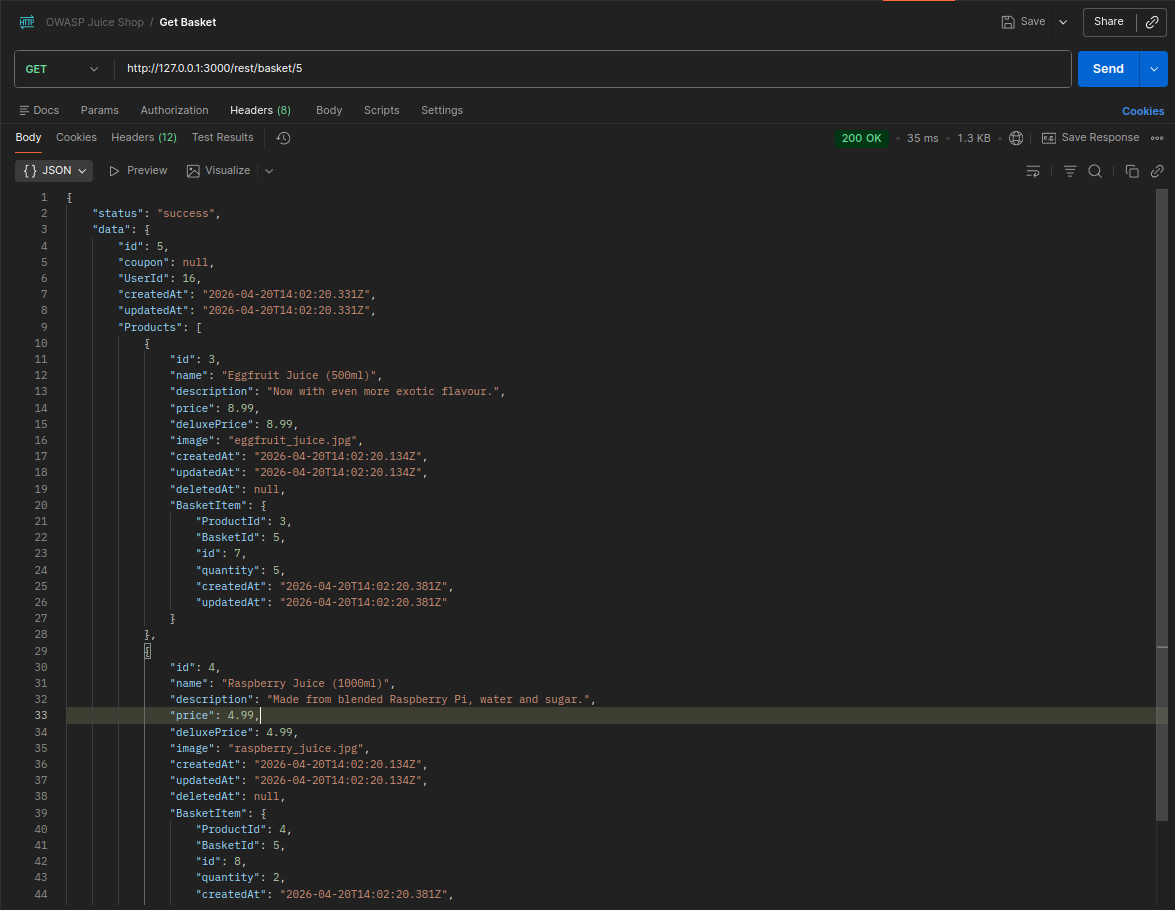
\includegraphics[width=1\textwidth]{images/access-control/postman.png}
            \caption{Postman request demonstrating broken access control by changing the Basket-ID in the URL to access another user's basket information. (Current user basket id is 6)}
            \label{fig:access-control-payload}
        \end{figure}

        \subsection{Remediation Recommendations}

        \begin{tcolorbox}[colback=lightgray,colframe=headerblack,title=\textbf{Recommended Fixes}]
        \textbf{1. Implement Proper Authorization Checks}

        Ensure that the server validates the user's session and JWT token against the requested Basket-ID to confirm that the user has permission to access that specific resource.

        \vspace{0.2cm}

        \textbf{2. Enforce Role-Based Access Control (RBAC)}

        Implement RBAC to restrict access to resources based on user roles and permissions, ensuring that users can only access their own data.

        \vspace{0.2cm}

        \textbf{3. Use Unique Identifiers}

        Consider using unique identifiers that are not easily guessable for resources like baskets, to make it harder for attackers to enumerate and access other users' data.
        \end{tcolorbox}







        \section{ 2FA Bypass via TOTP Secret Exposure}


        \begin{tcolorbox}[colback=lightgray,colframe=headerblack,title=\textbf{Vulnerability Overview}]
        \begin{tabular}{>{\bfseries}p{5cm} p{10cm}}
        Vulnerability Class & Authentication \\

        Location & Database and Login Panel \\

        CVSS v4 Score & 8.9 (High) \\

        MITRE ATT\&CK & Tactic: Credential Access \\
                    & ID: T1555 (Credentials from Password Stores) \\
        \end{tabular}
        \end{tcolorbox}

        \vspace{0.4cm}

        \subsection{Root Cause}

        Due to the presence of other vulnerabilities in the system, it is possible to extract sensitive user data directly from the database. Among this data is the TOTP secret used for two-factor authentication (2FA), which is stored in plaintext without any form of encryption or protection.

        Because the secret is not encrypted, an attacker can easily import it into a standard 2FA application (e.g., Google Authenticator) and generate valid one-time passwords for the victim account.

        \vspace{0.3cm}

        \subsection{Impact Analysis}

        This vulnerability compromises authentication mechanisms and allows full account takeover:

        \begin{longtable}{|p{4cm}|p{10cm}|}
        \hline
        \rowcolor{lightgray}
        \textbf{Security Property} & \textbf{Impact} \\
        \hline

        Confidentiality & Exposure of TOTP secrets enables attackers to impersonate users. \\
        \hline

        Integrity & Unauthorized access allows attackers to modify user data and system state. \\
        \hline

        Availability & Accounts may be locked or abused, impacting legitimate user access. \\
        \hline

        \end{longtable}

        \vspace{0.3cm}

        \subsection{Evidence}

        The TOTP secret was retrieved from the database in plaintext format. The field storing the secret was not protected or encrypted, allowing direct reuse in a 2FA application.

        \begin{figure}[H]
            \centering
            
\includegraphics[width=0.9\textwidth]{images/totp/postman.png}
            \caption{Postman request demonstrating the leakage of the TOTP secret from the database if a user has 2FA enabled. "price" field contains the TOTP secret in plaintext, which can be imported into a 2FA app to generate valid one-time passwords.}
            \label{fig:totp-payload}
        \end{figure}

        \vspace{0.3cm}

        \subsection{Remediation Recommendations}

        \begin{tcolorbox}[colback=lightgray,colframe=headerblack,title=\textbf{Recommended Fixes}]

        \textbf{1. Encrypt TOTP Secrets}

        Store TOTP secrets securely using strong encryption (e.g., AES with proper key management). Secrets must never be stored in plaintext.

        \end{tcolorbox}

        \vspace{0.2cm}

        \section{JWT Token Forgery}

        \begin{tcolorbox}[colback=lightgray,colframe=headerblack,title=\textbf{Vulnerability Overview}]
        \begin{tabular}{>{\bfseries}p{5cm} p{10cm}}
        Vulnerability Class & Vulnerable Component \\

        Location & JW Token, Server \\

        CVSS v4 Score & 9.3 (Critical) \\

        MITRE ATT\&CK & Tactic: Credential Access \\
                    & ID: T1606 (Forge Web Credentials) \\
        \end{tabular}
        \end{tcolorbox}

        \vspace{0.4cm}

        \subsection{Root Cause}

        The application uses JSON Web Tokens (JWT) for authentication, but the implementation is flawed. The server does not properly verify the signature of the JWT tokens, allowing attackers to forge tokens with arbitrary payloads. By crafting a JWT with a manipulated payload (e.g., changing the userId to 1), an attacker can gain unauthorized access to the system as if they were the user with that ID.

        \vspace{0.3cm}

        \subsection{Impact Analysis}

        This vulnerability has a critical impact on the security of the application, as it allows attackers to bypass authentication and gain unauthorized access to user accounts and sensitive data.

        \begin{longtable}{|p{4cm}|p{10cm}|}
        \hline
        \rowcolor{lightgray}
        \textbf{Security Property} & \textbf{Impact} \\
        \hline
        Confidentiality & Attackers can access sensitive user data by forging JWT tokens. \\
        \hline
        Integrity & Attackers can impersonate users and perform unauthorized actions. \\
        \hline
        Availability & Compromised accounts may lead to abuse and service disruption. \\
        \hline
        \end{longtable}

        \vspace{0.3cm}

        \subsection{Evidence}

        JWT tokens were successfully forged by manipulating the payload and bypassing signature verification, granting unauthorized access to user accounts.

        \begin{figure}[H]
            \centering
            
\includegraphics[width=0.9\textwidth]{images/jwt/postman.png}
            \caption{Postman request demonstrating the forging of a JWT token to gain unauthorized access to a user account.}
            \label{fig:jwt-forgery}
        \end{figure}

        \vspace{0.3cm}

        \subsection{Remediation Recommendations}

        \begin{tcolorbox}[colback=lightgray,colframe=headerblack,title=\textbf{Recommended Fixes}]
        \textbf{1. Enforce JWT Signature Verification (Critical)}

        Ensure that the server strictly verifies JWT signatures and rejects insecure configurations such as tokens using \textbf{"alg": "none"} and untrusted or unspecified algorithms
        
        \vspace{0.2cm}

        Explicitly whitelist secure algorithms (e.g., \texttt{HS256}, \texttt{RS256}):


        \textit{Never rely on the algorithm specified in the token header.}

        \vspace{0.2cm}

        \textbf{2. Use Strong Signing Keys}

        Use cryptographically strong keys for signing tokens

        \vspace{0.2cm}

        \textbf{3. Do Not Trust Token Claims Alone}

        Always validate token contents against the server-side state:

        \begin{itemize}
            \item Verify that \texttt{userId} exists
            \item Ensure the user account is active
            \item Validate authorization roles and permissions
        \end{itemize}

        \textit{JWTs should be treated as input, not as a source of truth.}

        \vspace{0.3cm}

        \textbf{4. Remove Sensitive Data from JWT Payload}

        Avoid including sensitive information inside JWTs. Password hashes, TOTP secrets, or any personally identifiable information (PII) should never be part of the token payload.

        \vspace{0.2cm}

\textbf{5. Implement Token Integrity \& Validation Checks}

Validate standard JWT claims to ensure token integrity with checks such as \texttt{exp} (expiration), \texttt{nbf} (not before), and \texttt{aud} (audience) to prevent replay attacks and ensure tokens are used within their intended context.

Ensure tokens are rejected if any of these validations fail.
        \end{tcolorbox}
        

    \chapter{Phase B Findings}

    \section{Attack Plan}
    \label{sec:attack-plan}

    \begin{table}[H]
    \centering
    \begin{tabular}{|p{4cm}|p{4cm}|p{6cm}|}
    \hline
    \textbf{Vulnerability Class} & \textbf{WSTG Test Case} & \textbf{Purpose} \\
    \hline
    Brute Force & \textbf{WSTG-ATHN-07} & Assess whether weak or predictable credentials can be discovered through password guessing or dictionary-based attacks. \\
    \hline
    Cross-Site Request Forgery (CSRF) & \textbf{WSTG-SESS-05} & Determine whether sensitive actions can be triggered without proper anti-CSRF protection. \\
    \hline
    SQL Injection & \textbf{WSTG-INPV-05} & Assess whether the application is vulnerable to SQL injection attacks. \\
    \hline
    Weak Session ID & \textbf{WSTG-SESS-02} & Evaluate the strength and uniqueness of session identifiers. \\
    \end{tabular}
    \caption{Planned vulnerability classes and associated WSTG test cases}
    \label{tab:wstg-plan}
    \end{table}

    \subsection{Brute Force Testing Plan}

    The first vulnerability class to be tested is Brute Force. The relevant WSTG test case is \textbf{WSTG-ATHN-07: Testing for Weak Password Policy}. The objective is to determine whether the DVWA login mechanism allows weak credentials to be guessed using a controlled dictionary or traditional brute-force approach.

    The hypothesis is that the Medium-level control can be bypassed by carefully analysing HTTP responses and automating requests at a controlled rate. Burp Suite may be used to intercept login attempts and compare differences between failed and successful responses. A small dictionary attack may be performed against known DVWA users, such as the default administrative account, while monitoring response content, status codes, redirects, and timing behaviour.

    \subsection{Cross-Site Request Forgery Testing Plan}

    The second vulnerability class to be tested is Cross-Site Request Forgery. The relevant WSTG test case is \textbf{WSTG-SESS-05: Testing for Cross Site Request Forgery}. The objective is to determine whether DVWA allows an attacker to force an authenticated user to perform a sensitive action without the user's explicit consent.

    The hypothesis is that the Medium-level control can be bypassed if the protection relies only on weak request validation, such as predictable request structure or insufficient referrer checking. Testing will involve capturing a legitimate password-change request, identifying whether an anti-CSRF token is present, and attempting to replay or reproduce the request from an external page or crafted link.

    \subsection{SQL Injection Testing Plan}

    The third vulnerability class to be tested is SQL Injection. The relevant WSTG test case is \textbf{WSTG-INPV-05: Testing for SQL Injection}. The objective is to determine whether the application is vulnerable to SQL injection attacks.

    The hypothesis is that the Medium-level control can be bypassed if the application does not properly sanitise or validate user input before executing database queries. Testing will involve submitting malicious SQL payloads through various input fields and analysing the application's response to identify potential vulnerabilities.

    \subsection{Weak Session ID Testing Plan}

    The fourth vulnerability class to be tested is Weak Session ID. The relevant WSTG test case is \textbf{WSTG-SESS-02: Testing for Weak Session IDs}. The objective is to evaluate the strength and uniqueness of session identifiers used by the application.

    The hypothesis is that the session management mechanism may generate predictable or weak session IDs that can be easily guessed or brute-forced by an attacker. Testing will involve analysing the session ID generation process, collecting multiple session IDs, and assessing their randomness and uniqueness using statistical methods.

    \section{Summary of Findings}
    \label{sec:phase-b-summary}

    \begin{table}[H]
    \centering
    \renewcommand{\arraystretch}{1.35}
    \begin{tabular}{|p{1.2cm}|p{4cm}|p{3.2cm}|p{2.2cm}|p{3cm}|}
    \hline
    \textbf{ID} & \textbf{Finding Title} & \textbf{Vulnerability Class} & \textbf{Severity} \\
    \hline
    B-01 & Vulnerable Login & Brute Force & Critical \\
    \hline
    B-02 & Cross-Site Request Forgery & CSRF & High \\
    \hline
    B-03 & SQL Injection & SQL Injection & Critical \\
    \hline
    B-04 & Weak Session IDs & Weak Session ID & Medium \\
    \hline
    \end{tabular}
    \caption{Summary of Phase B findings}
    \label{tab:phase-b-summary}
    \end{table}

    \section{Finding B-01: Vulnerable Login}
    \label{sec:finding-b01}

    \subsection*{Vulnerability Class}
    Brute Force

    \subsection*{Description}
    It's possible to brute force the login page at Medium security level. The login form does not implement any effective lockout mechanism, rate limiting, or account protection controls. This allows an attacker to automate login attempts using a dictionary of common passwords or brute-force techniques without being blocked or delayed by the application.

    \subsection*{Medium-Security Control Observed}
    The medium security level of DVWA implements just a 2 seconds delay after each failed login attempt, which is insufficient to prevent brute-force attacks. There are no account lockouts, CAPTCHA challenges, or IP-based rate limiting in place to deter automated login attempts.

    \subsection*{Bypass Hypothesis}
    The hypothesis is that by using an automated tool like Burp Suite's Intruder, an attacker can submit a large number of login attempts with different password combinations while only experiencing a minimal delay of 2 seconds per attempt. This allows for efficient brute-force testing against the login form, especially if the attacker has a list of common passwords or known credentials to test against.

    \subsection*{Evidence}

    \subsubsection*{Screenshot Evidence}
    \begin{figure}[H]
        \centering
        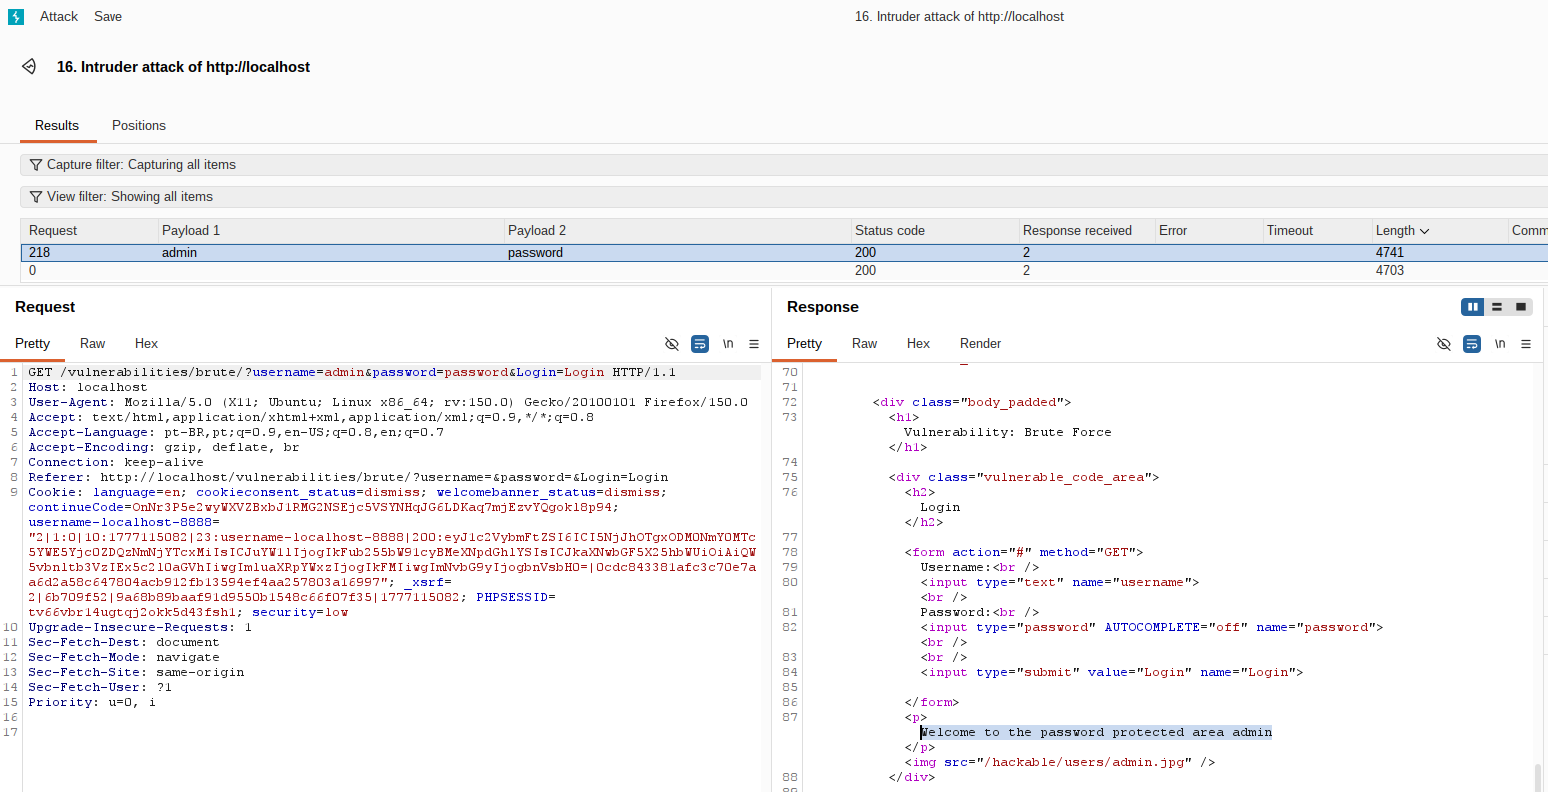
\includegraphics[width=1\textwidth]{images/burp/image.png}
        \caption{Request and Response in Burp Suite Intruder with successful brute-force login attempt.}
        \label{fig:finding-b01-evidence}
    \end{figure}

    \subsection*{Steps to Reproduce}
    \begin{enumerate}
        \item Try to login to get the complete request in Burp Suite.
        \item Send the login request to Intruder and configure a payload list with common passwords or a dictionary of passwords.
        \item Set the attack type to "Sniper" or "Cluster Bomb" depending on the payload configuration.
        \item Start the attack and observe the Length of responses to identify successful login attempts. 
    \end{enumerate}

    \subsection*{Impact}
    This vulnerability allows attackers to gain unauthorized access to user accounts, including potentially administrative accounts, by systematically guessing passwords. Once an account is compromised, the attacker can access sensitive information, perform actions on behalf of the user, and potentially escalate privileges if the compromised account has administrative rights.

    \newpage
    \subsection*{Logs}
    \begin{table}[h!]
    \centering
    \renewcommand{\arraystretch}{1.3}
    \begin{tabular}{|p{4cm}|p{9cm}|}
    \hline
    Timestamp & \texttt{2026-05-2T14:23:11Z} \\
    \hline
    Source IP & \texttt{89.154.80.19} \\
    \hline
    Destination IP & \texttt{127.0.0.1} \\
    \hline
    Destination Port & \texttt{80} \\
    \hline
    Technique & \texttt{T1110} \\
    \hline
    Tactic & Credential Access \\
    \hline
    Tool & \texttt{Burp Suite Community Edition Intruder} \\
    \hline
    Payload & \texttt{admin:password} \\
    \hline
    Outcome & \textbf{Success} \\
    \hline
    Finding Reference & \texttt{B-01} \\
    \hline
    Observable & HTTP 200 with length 4741 \\
    \hline
    \end{tabular}
    \end{table}

    \section{Finding B-02: Cross-Site Request Forgery}
    \label{sec:finding-b02}

    \subsection*{Vulnerability Class}
    Cross-Site Request Forgery (CSRF)

    \subsection*{Description}
    The application does not implement proper anti-CSRF tokens or protections on sensitive actions, such as changing a user's password. This allows an attacker to craft a malicious request that, when executed by an authenticated user, can perform actions on their behalf without their consent.
    
    \subsection*{Medium-Security Control Observed}
    There is a check to see where the last requested page came from, the Referrer header. However, this is not a reliable method of protection against CSRF attacks, as the Referrer header can be easily spoofed or omitted by attackers. Additionally, relying solely on the Referrer header does not provide robust protection against CSRF, as it does not verify the legitimacy of the request or the user's intent.

    \subsection*{Bypass Hypothesis}
    The hypothesis is that by crafting a malicious HTML form or using a tool like Burp Suite, an attacker can create a request that mimics a legitimate password change request. By setting the Referrer header to match the expected value, the attacker can bypass the weak CSRF protection and successfully change the user's password without their knowledge.

    \subsection*{Evidence}
    \subsubsection*{Request}
    \begin{lstlisting}[language=bash]
http://localhost/vulnerabilities/csrf/?password_new=olaa&password_conf=olaa&Change=Change
    \end{lstlisting}

    \subsubsection*{Screenshot Evidence}
    \begin{figure}[H]
        \centering
        
\includegraphics[width=1\textwidth]{images/csrf/image.png}
        \caption{Browser launching a crafted request to change the password, with the Referrer header set to bypass the CSRF protection.}
        \label{fig:finding-b02-evidence}
    \end{figure}


    \begin{figure}[H]
        \centering
        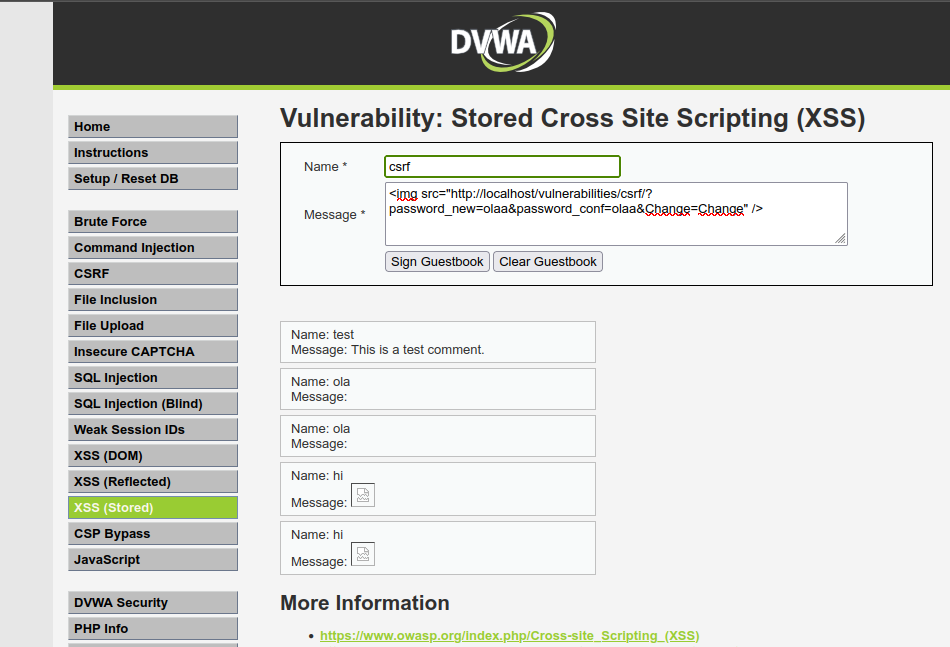
\includegraphics[width=1\textwidth]{images/csrf/image2.png}
        \caption{Creating a csrf from xss}
        \label{fig:finding-b02-evidence-xss}
    \end{figure}

    \subsection*{Steps to Reproduce}
    \begin{enumerate}
        \item Forge a request to the password change endpoint with the necessary parameters (e.g., \texttt{password\_new}, \texttt{password\_conf}, and \texttt{Change}).
        \item Find a way to set the Referrer header to match the expected value (e.g., by hosting a malicious HTML page or exploiting another vulnerability in the website).
        \item Have an authenticated user visit the malicious page or trigger the crafted request, which will then execute the password change action without the user's consent.
        \item Observe that the password has been changed successfully, confirming the CSRF vulnerability.
    \end{enumerate}

    \subsection*{Impact}
    This vulnerability allows attackers to perform unauthorized actions on behalf of authenticated users, such as changing their password. This can lead to account compromise, loss of access for the legitimate user, and potential further exploitation if the attacker can gain control over the account.

    \subsection*{Logs}
    
    \begin{table}[h!]
    \centering
    \renewcommand{\arraystretch}{1.3}
    \begin{tabular}{|p{4cm}|p{9cm}|}
    \hline
    Timestamp & \texttt{2026-05-3T21:53:11Z} \\
    \hline
    Source IP & \texttt{89.154.80.19} \\
    \hline
    Destination IP & \texttt{127.0.0.1} \\
    \hline
    Destination Port & \texttt{80} \\
    \hline
    Technique & \texttt{T1098} \\
    \hline
    Tactic & Account Manipulation \\
    \hline
    Tool & \texttt{Burp Suite Community Edition Proxy} \\
    \hline
    Payload & \texttt{...=olaa\&password\_conf=olaa\&Change=Change} \\
    \hline
    Outcome & \textbf{Success} \\
    \hline
    Finding Reference & \texttt{B-02} \\
    \hline
    Observable & Response "Password changed" \\
    \hline
    \end{tabular}
    \end{table}

    \newpage

    \section{Finding B-03: SQL Injection}
    \label{sec:finding-b03}

    \subsection*{Vulnerability Class}
    SQL Injection

    \subsection*{Description}
    The application is vulnerable to SQL injection attacks, allowing an attacker to manipulate database queries by injecting malicious SQL code through user input fields. This can lead to unauthorized access to data, data manipulation, or even complete compromise of the database.

    Given that the source code of DVWA shows a vulnerable SQL query that directly incorporates user input without proper sanitization, it is likely that the application does not implement effective controls to prevent SQL injection. The query in question is:

    \begin{lstlisting}[
        style=phpstyle,
        caption={Source code from DVWA illustrating the vulnerable SQL query},
        label={lst:sqli-code}
    ]
    $query = "SELECT first_name, last_name FROM users WHERE user_id = $id;";
    \end{lstlisting}

    A malicious user can manipulate the \texttt{\$id} variable by injecting SQL code, which can lead to various malicious outcomes such as data exfiltration, data modification, or even remote code execution if the database is configured to allow it.

    \subsection*{Medium-Security Control Observed}
    The medium security level of DVWA implements basic input sanitization, which may prevent some simple SQL injection attempts. However, this control is not robust and can be bypassed with more sophisticated payloads that evade the sanitization filters. 
    Also, it was recognized that instead of an input field, the injection point is through a dropbox that allows the user to select an ID. This may give a false sense of security, as it may appear that the input is controlled and limited to valid IDs. However, if the application does not properly validate or sanitize the selected ID before using it in the SQL query, it can still be vulnerable to SQL injection attacks by just manipulating the HTML structure.

    \subsection*{Bypass Hypothesis}
    The hypothesis is that by crafting a more complex SQL injection payload that can bypass the basic sanitization, an attacker can successfully execute arbitrary SQL commands against the database. This may involve using techniques such as encoding, comment-based obfuscation, or leveraging specific database functions to achieve the desired outcome.

    \subsection*{Evidence}
    \subsubsection*{Request}
    \begin{lstlisting}[language=bash, caption={SQL injection payload used to bypass the Medium security control}]
    1 OR 1=1 UNION SELECT user,password FROM users
    \end{lstlisting}

    \subsubsection*{Screenshot Evidence}
    \begin{figure}[H]
        \centering
        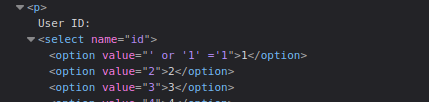
\includegraphics[width=0.85\textwidth]{images/sql/html.png}
        \caption{Modified HTML structure to inject SQL code through the dropbox selection.}
        \label{fig:finding-b03-evidence}
    \end{figure}

    \begin{figure}[H]
        \centering
        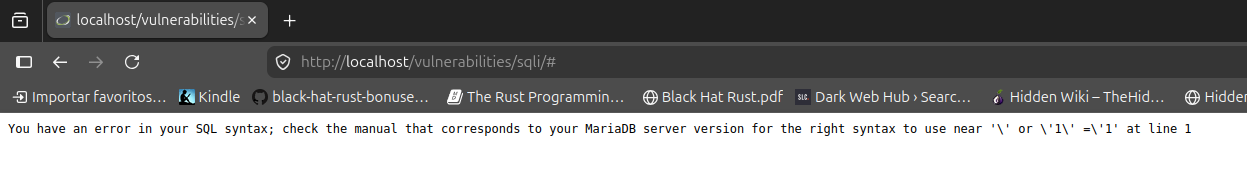
\includegraphics[width=0.85\textwidth]{images/sql/error.png}
        \caption{Error message indicating successful SQL injection.}
        \label{fig:finding-b03-evidence-2}
    \end{figure}

    \begin{figure}[H]
        \centering
        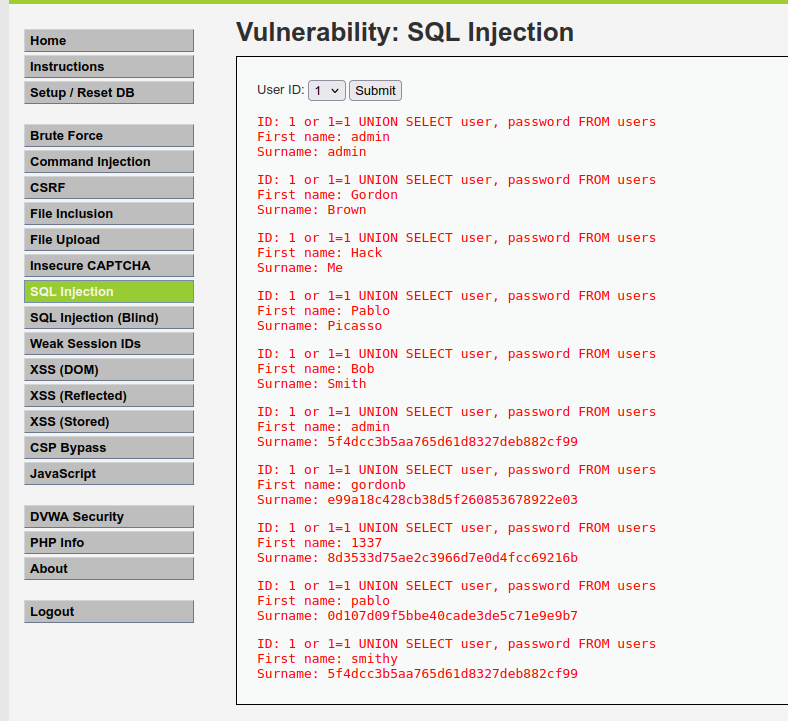
\includegraphics[width=0.85\textwidth]{images/sql/success.png}
        \caption{Success message indicating successful SQL injection.}
        \label{fig:finding-b03-evidence-3}
    \end{figure}


    \subsection*{Steps to Reproduce}
    \begin{enumerate}
        \item Inspect the HTML structure of the page to identify the dropbox element that allows selection of user IDs.
        \item Modify the HTML structure to inject a malicious SQL payload into the dropbox selection.
        \item Submit the modified request and observe the response for signs of successful SQL injection, such as error messages or unexpected data being returned.
        \item Iterate on the payload as needed to bypass the sanitization and achieve the desired outcome (e.g., retrieving user credentials).
    \end{enumerate}

    \subsection*{Impact}
    This vulnerability allows attackers to execute arbitrary SQL commands against the database, which can lead to unauthorized access to sensitive data, data manipulation, or even complete compromise of the database. The impact can be severe, especially if the database contains critical information or if the attacker can leverage the SQL injection to gain further access to the system.

    \subsection*{Logs}
    
     \begin{table}[h!]
    \centering
    \renewcommand{\arraystretch}{1.3}
    \begin{tabular}{|p{4cm}|p{9cm}|}
    \hline
    Timestamp & \texttt{2026-05-5T16:53:11Z} \\
    \hline
    Source IP & \texttt{89.154.80.19} \\
    \hline
    Destination IP & \texttt{127.0.0.1} \\
    \hline
    Destination Port & \texttt{80} \\
    \hline
    Technique & \texttt{T1190} \\
    \hline
    Tactic & Exploit Public-Facing Application \\
    \hline
    Tool & \texttt{Firefox} \\
    \hline
    Payload & \texttt{'1 OR '1'='1} \\
    \hline
    Outcome & \textbf{Error - SQL Injection Attempt} \\
    \hline
    Finding Reference & \texttt{B-03} \\
    \hline
    Observable & Error message indicating SQL injection attempt \\
    \hline
    \end{tabular}
    \end{table}

    \begin{table}[h!]
    \centering
    \renewcommand{\arraystretch}{1.3}
    \begin{tabular}{|p{4cm}|p{9cm}|}
    \hline
    Timestamp & \texttt{2026-05-5T17:20:11Z} \\
    \hline
    Source IP & \texttt{89.154.80.19} \\
    \hline
    Destination IP & \texttt{127.0.0.1} \\
    \hline
    Destination Port & \texttt{80} \\
    \hline
    Technique & \texttt{T1190} \\
    \hline
    Tactic & Exploit Public-Facing Application \\
    \hline
    Tool & \texttt{Firefox} \\
    \hline
    Payload & \texttt{1 OR 1=1 UNION SELECT user,password FROM users} \\
    \hline
    Outcome & \textbf{Success - SQL Injection} \\
    \hline
    Finding Reference & \texttt{B-03} \\
    \hline
    Observable & Success message indicating SQL injection \\
    \hline
    \end{tabular}
    \end{table}

    \newpage

    \section{Finding B-04: Weak Session IDs}
    \label{sec:finding-b04}

    \subsection*{Vulnerability Class}
    Weak Session ID

    \subsection*{Description}
    The application generates session identifiers that are weak and predictable, making it possible for attackers to guess or brute-force valid session IDs. This can lead to session hijacking, where an attacker can impersonate a legitimate user by using a valid session ID.

    It was concluded that the session Ids are generated using UNIX timestamps, which are predictable and can be easily guessed by an attacker. This means that an attacker can generate valid session IDs by simply creating them based on the timestamp, allowing them to hijack active sessions and gain unauthorized access to user accounts.
    
    \subsection*{Medium-Security Control Observed}
    The medium security level of DVWA does not implement any robust controls to ensure the randomness and uniqueness of session IDs. The use of predictable session ID generation methods, such as using timestamps, is a significant weakness that can be easily exploited by attackers.

    \subsection*{Bypass Hypothesis}
    The hypothesis is that by analyzing the session ID generation mechanism, an attacker can predict valid session IDs based on the current time and successfully hijack active sessions. This can be done by generating session IDs that correspond to recent timestamps and using them to access the application as if they were a legitimate user.

    \subsection*{Evidence}
    \subsubsection*{Request}
    \begin{lstlisting}[language=bash, caption={HTTP request or command used for Finding B-04}]
    POST /vulnerabilities/weak_id/ HTTP/1.1
    Host: localhost
    User-Agent: Mozilla/5.0 (X11; Ubuntu; Linux x86_64; rv:150.0) Gecko/20100101 Firefox/150.0
    ...
    Connection: keep-alive
    Referer: http://localhost/vulnerabilities/weak_id/
    Cookie: dvwaSession=1778062783; ...
    ...
    \end{lstlisting}

    \subsubsection*{Response}
    \begin{lstlisting}[language=html, caption={Relevant response evidence for Finding B-04}]
    HTTP/1.1 200 OK
    ...
    Set-Cookie: dvwaSession=1778062886
    ...
    \end{lstlisting}

    \subsubsection*{Screenshot Evidence}
    \begin{figure}[H]
        \centering
        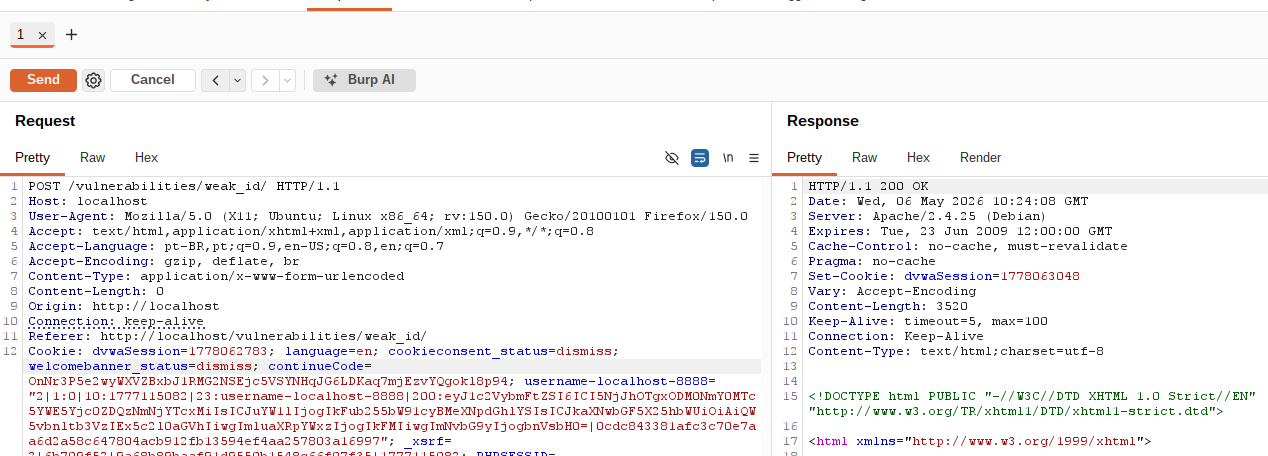
\includegraphics[width=0.85\textwidth]{images/id/first.png}
        \caption{Session ID with a predictable value based on the timestamp.}
    \end{figure}

    \begin{figure}[H]
        \centering
        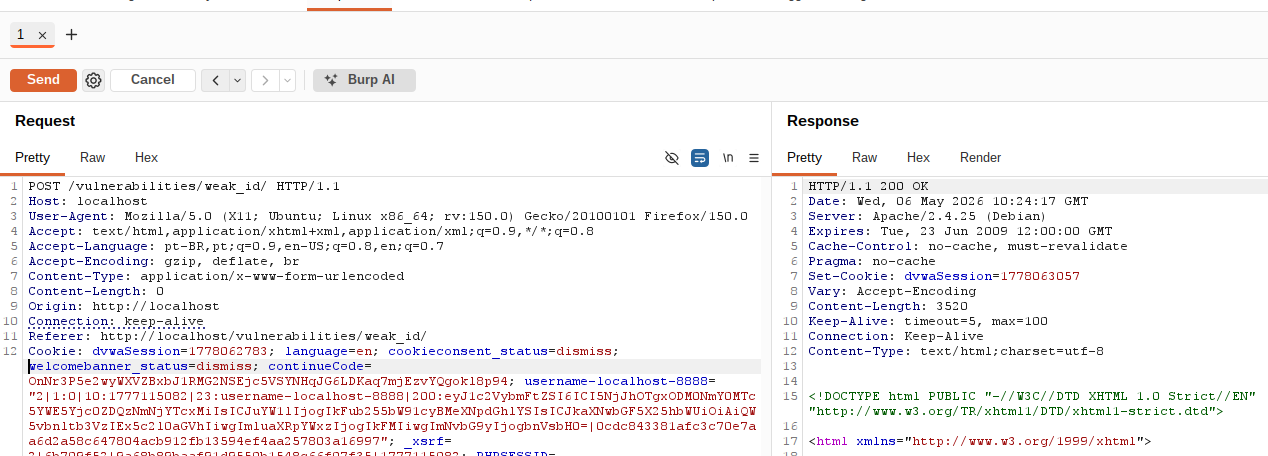
\includegraphics[width=0.85\textwidth]{images/id/second.png}
        \caption{dvwaSession=1778063057, 10 seconds after the first session ID, demonstrating the predictable nature of the session IDs.}
    \end{figure}

    \subsection*{Steps to Reproduce}
    \begin{enumerate}
        \item Analyze the session ID generation mechanism to understand how session IDs are created (e.g., using timestamps).
        \item Generate valid session IDs based on the current time or recent timestamps.
        \item Use the generated session IDs to attempt to access the application and hijack active sessions.
    \end{enumerate}

    \subsection*{Impact}
    This vulnerability allows attackers to hijack active sessions by predicting valid session IDs, leading to unauthorized access to user accounts and sensitive information. The impact can be significant, especially if the attacker can gain access to administrative accounts or accounts with elevated privileges.

    \newpage
    
    \subsection*{Logs}

    \begin{table}[h!]
    \centering
    \renewcommand{\arraystretch}{1.3}
    \begin{tabular}{|p{4cm}|p{9cm}|}
    \hline
    Timestamp & \texttt{2026-05-6T11:10:11Z} \\
    \hline
    Source IP & \texttt{89.154.80.19} \\
    \hline
    Destination IP & \texttt{127.0.0.1} \\
    \hline
    Destination Port & \texttt{80} \\
    \hline
    Technique & \texttt{T1185} \\
    \hline
    Tactic & Browser Session Hijacking \\
    \hline
    Tool & \texttt{Firefox} \\
    \hline
    Payload & \texttt{[UNIX Timestamp]} \\
    \hline
    Outcome & \textbf{Success} \\
    \hline
    Finding Reference & \texttt{B-04} \\
    \hline
    Observable & Server Response Success \\
    \hline
    \end{tabular}
    \end{table}

    \newpage

    \chapter{Cross-Phase Analysis}

        \begin{tcolorbox}[
            colback=lightgray,
            colframe=headerblack,
            title=\textbf{Cross-Phase View},
            arc=1mm,
            boxrule=0.8pt
        ]
        Phase A built the testing method; Phase B tested whether that method still worked when basic defences were added. The strongest transfer was not a payload, but the workflow: capture normal behaviour, change one trusted value, and prove the impact with evidence.
        \end{tcolorbox}

        \vspace{0.25cm}

        \begin{table}[H]
        \centering
        \renewcommand{\arraystretch}{1.55}
        \begin{tabular}{|p{3.1cm}|p{5.0cm}|p{5.0cm}|}
        \hline
        \rowcolor{black!85}
        \textcolor{white}{\textbf{Theme}} &
        \textcolor{white}{\textbf{Phase A: Juice Shop}} &
        \textcolor{white}{\textbf{Phase B: DVWA Medium}} \\
        \hline
        \cellcolor{blue!10}\textbf{Direct transfer} &
        SQL injection in \texttt{/rest/products/search}; basket ID manipulation through the API. &
        SQL injection B-03; request replay and modification in B-01, B-02, and B-04. \\
        \hline
        \cellcolor{orange!15}\textbf{Adaptation needed} &
        Exploits were mostly direct once the vulnerable endpoint was understood. &
        Dropdown input, referrer checks, login delay, and predictable session IDs required request/HTML manipulation. \\
        \hline
        \cellcolor{red!10}\textbf{Security lesson} &
        Server trusted attacker-controlled identifiers, secrets, and JWT claims. &
        Medium controls slowed testing but did not enforce strong server-side trust decisions. \\
        \hline
        \end{tabular}
        \caption{Comparison of technique transfer and adaptation across both phases}
        \end{table}

        \vspace{0.2cm}

        \noindent
        \begin{minipage}[t]{0.48\textwidth}
        \begin{tcolorbox}[
            colback=lightgray!5,
            colframe=headerblack,
            title=\textbf{What Transferred},
            arc=1mm
        ]
        \begin{itemize}[leftmargin=*, itemsep=0.1cm]
            \item Request interception and replay
            \item Parameter tampering
            \item SQL injection reasoning
            \item Evidence-first validation
        \end{itemize}
        \end{tcolorbox}
        \end{minipage}
        \hfill
        \begin{minipage}[t]{0.48\textwidth}
        \begin{tcolorbox}[
            colback=lightgray!5,
            colframe=headerblack,
            title=\textbf{What Changed},
            arc=1mm
        ]
        \begin{itemize}[leftmargin=*, itemsep=0.1cm]
            \item Payloads needed adjustment
            \item Client controls had to be bypassed
            \item Headers and session values mattered more
            \item Automation had to account for delays
        \end{itemize}
        \end{tcolorbox}
        \end{minipage}

        \vspace{0.35cm}

        \begin{tcolorbox}[
            colback=lightgray!5,
            colframe=headerblack,
            title=\textbf{Main Defensive Conclusion},
            arc=1mm,
            boxrule=0.8pt
        ]
        DVWA's medium controls were useful but incomplete: dropdowns, referrer checks, predictable session values, and small login delays make exploitation less convenient, but they do not remove the vulnerability. Real protection must happen on the server through parameterised queries, strict authorisation checks, strong session generation, verified tokens, protected secrets, and action-specific CSRF tokens.
        \end{tcolorbox}

    \chapter{Conclusion}
        
        This report has demonstrated the importance of understanding the underlying vulnerabilities and attack techniques, rather than relying solely on specific payloads or tools. The transfer of techniques from Phase A to Phase B required adaptation to the new environment and controls, but the core principles of exploitation and evidence gathering remained consistent.

        The findings highlight that while basic security controls can slow down attackers, they are not sufficient to prevent exploitation if the underlying vulnerabilities are not properly addressed. Effective security requires a comprehensive approach that includes secure coding practices, robust input validation, proper session management, and strong authentication mechanisms. By focusing on the root causes of vulnerabilities and implementing strong server-side protections, organizations can significantly reduce the risk of successful attacks and protect their users' data and privacy.

\end{document}
